\section{Overview}

    \begin{figure}[H]
        \centering
        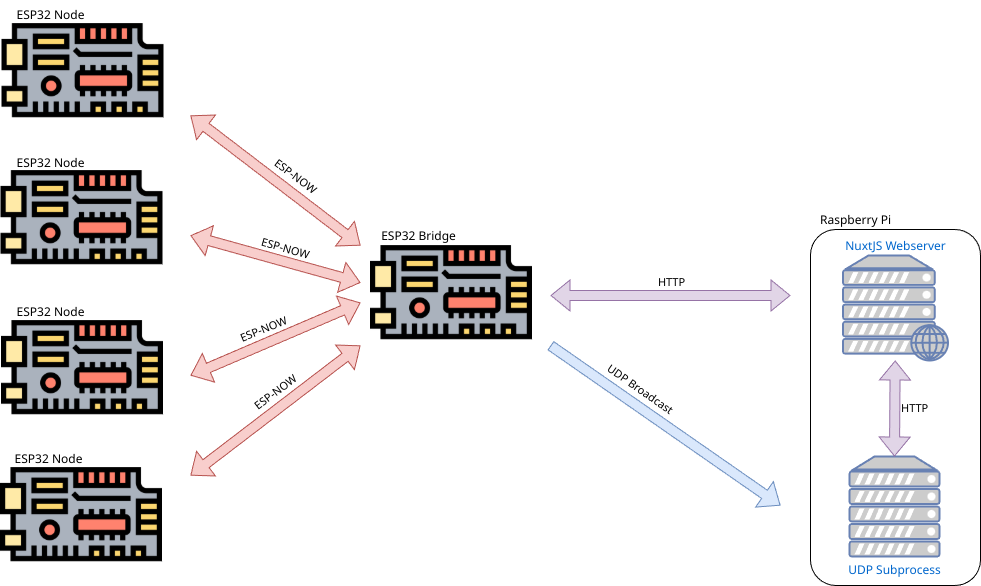
\includegraphics[width=0.9\textwidth]{topics/flowcharts/Networking.png}
        \caption{Networking Structure}
    \end{figure}
    \subsection{Web Server}
    A Nuxt.js Web server will function as the main interface
    for the user. It will communicate with the database and the
    dedicated Bridge-Node via HTTP. It should be capable of displaying
    and changing the state of the devices in the smart home.
    \subsection{Bridge-Node}
    The Bridge-Node will act as a bridge between everything running
    on the Raspberry Pi (Web server, database) and the ESP-NOW devices.
    It will be capable of receiving and sending data via both HTTP and
    ESP-NOW. It will also be responsible for discovering new ESP-NOW
    devices.
    \subsection{Slave-Nodes}
    The Slave-Nodes will be the ESP32 devices. They will be capable of
    sending and receiving data via ESP-NOW to and from the Bridge-Node.
    This only happens when a request is made by the Bridge-Node. Due to 
    the fact that the Bridge only sends a request when the user interacts
    with the Web server, all Slave traffic is triggered by the Webserver.
    Note that this excludes the discovery process (see section \ref{sec:espnow_discovery}).
